\documentclass[11pt]{article}
\usepackage[margin=.78in]{geometry}
\usepackage[T1]{fontenc}
\usepackage{lmodern}
\usepackage{xcolor,listings,booktabs,amsmath,amssymb,hyperref,enumitem,tikz}
\usetikzlibrary{arrows.meta,positioning}
\hypersetup{colorlinks=true,linkcolor=blue!55!black,urlcolor=blue!55!black}
\definecolor{codebg}{HTML}{F5F7FA}
\definecolor{codeblue}{HTML}{2457A6}
\definecolor{codegreen}{HTML}{287A48}
\definecolor{codestring}{HTML}{A33A20}
\lstdefinestyle{python}{language=Python,basicstyle=\ttfamily\footnotesize,keywordstyle=\color{codeblue}\bfseries,commentstyle=\color{codegreen}\itshape,stringstyle=\color{codestring},showstringspaces=false,breaklines=true,frame=single,rulecolor=\color{black!18},backgroundcolor=\color{codebg},numbers=left,numberstyle=\tiny\color{black!45},numbersep=7pt,upquote=true,columns=fullflexible}
\title{An EDSL-Defined Loop for School Choice\\\large The Machine's State, Iteration, and Execution}
\author{Technical note for the LLM preference pilot}
\date{October 11, 2026}
\begin{document}
\maketitle

\begin{abstract}
This note documents the revised school-choice Machine, in which deferred acceptance's proposer selection, proposal construction, state update, and stop condition are all represented as EDSL data expressions. A generic EDSL Runtime initializes the Machine and applies its standard close transition; the close effect evaluates a bounded \texttt{iterate} expression until the matching algorithm's stop condition holds. There is no experiment-specific Python loop selecting proposals. The Machine remains JSON-serializable and declares no Python algorithm callbacks. This design is an important step toward submitting an experiment to a generic remote executor: market-specific procedure is now in the serialized definition, while the EDSL interpreter remains the shared execution engine.
\end{abstract}

\section{The change in one sentence}
The earlier version exposed one command per proposal and left Python to select each next proposer. The current version puts the complete deferred-acceptance loop inside the Machine's \texttt{close\_effects}: an EDSL \texttt{iterate} repeatedly chooses the next proposer, computes the proposal transition, and stops when no proposer remains eligible. The experiment runner now just constructs a Machine, initializes the generic Runtime, and invokes the standard close operation.

\begin{figure}[h]
\centering
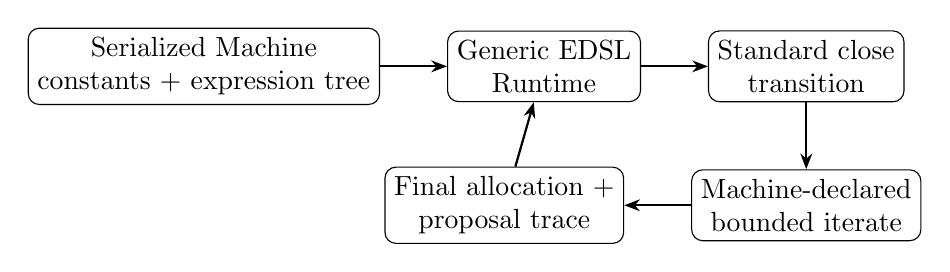
\begin{tikzpicture}[node distance=.85cm,every node/.style={draw,rounded corners,align=center,minimum width=2.45cm,minimum height=.7cm},arr/.style={-{Stealth[length=2mm]},thick}]
\node (spec) {Serialized Machine\\constants + expression tree};
\node[right=of spec] (runtime) {Generic EDSL\\Runtime};
\node[right=of runtime] (close) {Standard close\\transition};
\node[below=of close] (loop) {Machine-declared\\bounded iterate};
\node[left=of loop] (result) {Final allocation +\\proposal trace};
\draw[arr] (spec)--(runtime); \draw[arr] (runtime)--(close); \draw[arr] (close)--(loop); \draw[arr] (loop)--(result); \draw[arr] (result)--(runtime);
\end{tikzpicture}
\caption{The generic Runtime executes the loop encoded in the Machine. Python no longer chooses each proposer.}
\end{figure}

\section{What is serialized}
\texttt{build\_machine} runs at authoring time. It selects one proposer side, validates the supplied student rankings, computes rank lookup maps, embeds preferences, capacities, and school priorities as constants, and constructs the expression tree for that side's loop. \texttt{Machine.to\_json()} serializes those constants and EDSL expressions; \texttt{algorithms=()} means no named Python callback is required to execute the mechanism.

\lstinputlisting[style=python,firstline=332,lastline=384,caption={Machine definition: serialized constants, state type, close effect, and completion condition}]{machine_definition.py}

The serialized definition is portable between EDSL runtimes that implement the declared Machine language version and expression capabilities. The destination does not need the school-choice Python source to interpret the transition tree. It does need a compatible generic EDSL interpreter. The result-producing expression runs through the standard Machine close operation rather than an application-specific command dispatcher.

\section{The state carried through iteration}
The live allocation is one typed record $x=(Q,A,H,n_S,n_C,L,f)$:
\begin{center}
\begin{tabular}{ll}
\toprule
Value & Interpretation \\
\midrule
$Q$ & student-proposing queue; unused by the school-proposing loop \\
$A:S\to C\cup\{\bot\}$ & current student assignments \\
$H:C\to 2^S$ & each school's tentative holds \\
$n_S:S\to\mathbb{N}$ & each student's next school index \\
$n_C:C\to\mathbb{N}$ & each school's next student-priority index \\
$L$ & ordered proposal log \\
$f$ & completion flag \\
\bottomrule
\end{tabular}
\end{center}

Initial state is all students unmatched, all school holds empty, both cursor maps zeroed, an empty proposal log, and $f=\text{false}$. In each iteration the accumulator is a complete allocation record. The EDSL \texttt{iterate} operation binds the current record to a local name, evaluates the stop predicate, and if false evaluates one pure step expression to produce the next record. The step has a declared record type, checked after every internal iteration. If its explicit step budget is exhausted before the condition becomes true, the Runtime raises an execution error; it never silently returns a partial allocation.

\section{Student-proposing loop}
At each iteration, $Q$ begins with the student IDs in fixed order. The step takes its first student $s$. If $s$ has exhausted their list, the step removes $s$ from $Q$. Otherwise it selects $c=\succ_s[n_S(s)]$, forms $H(c)\cup\{s\}$, sorts those candidates by $c$'s priority rank, and retains the first $q_c$. It updates assignments and holds, advances $n_S(s)$, records the proposal, then puts rejected candidates at the end of $Q$. The loop stops when $Q$ is empty.

\lstinputlisting[style=python,firstline=106,lastline=237,caption={Student-proposing loop as EDSL expressions, including queue choice, proposal effects, and stop condition}]{machine_definition.py}

Each proposal consumes one student ranking position. A student can have at most one final queue visit after exhausting their list. Therefore the machine derives a safe bound
\[
  B_S=\sum_{s\in S}|\succ_s|+|S|.
\]
The bound is data-dependent and encoded as an expression over the serialized constants. It covers all proposals plus any final exhaustion visits.

\section{School-proposing loop}
At each iteration, the Machine filters schools in their declared order, keeping schools with an open seat and an untried student in their priority list. It selects the first active school $c$, then $s=\succ_c[n_C(c)]$. Student $s$ accepts if unmatched or if they prefer $c$ to their current assignment. An accepted offer updates $A$ and both affected schools' hold sets; a rejection leaves assignments and holds unchanged. The school's cursor advances either way, and the event is appended to $L$. Iteration stops when the active-school sequence is empty.

\lstinputlisting[style=python,firstline=240,lastline=329,caption={School-proposing loop as EDSL expressions, including eligibility selection and student choice}]{machine_definition.py}

Every school can propose to each student no more than once, so the loop has the finite upper bound
\[
  B_C=|C|\,|S|.
\]
The stop predicate checks the current allocation for any school that has both remaining capacity and an untried priority candidate. The loop does not rely on a Python scheduler to make this eligibility decision.

\section{Generic execution boundary}
The run driver now performs only generic lifecycle operations:

\lstinputlisting[style=python,firstline=14,lastline=26,caption={Generic initialization and close; there is no proposal-selection loop}]{run_pilot.py}

The close effect is atomic at the shared-state transition boundary: the Runtime evaluates the bounded loop against an internal accumulator and commits the resulting allocation as the close transition. The proposal log remains available in the final allocation for inspection. Intermediate matching states are not separately committed or externally observable during this close operation. That is a deliberate trade-off for this pilot: the whole matching is a pure, portable expression, while crash-resumable checkpoints between proposals would require a future resumable-iteration protocol.

The LLM interview is upstream of the Machine. It produces rankings that are validated and stored as constants. Provider calls, ranking normalization, and output analysis are not hidden inside the matching loop. For the LLM pilot the same saved profile and priority seed are embedded in both proposer-side definitions.

\section{Observed experiment results}
The preference pilot used twelve authored student personas, four school descriptions, and one \texttt{gpt-4o-mini} ranking interview per persona. School priorities use seed 42017. Both Machine instances executed through the new close-time loop.

\begin{center}
\begin{tabular}{lrr}
\toprule
Outcome & Student-proposing & School-proposing \\
\midrule
First choices assigned & 12 / 12 & 7 / 12 \\
Mean student rank, 1 = best & 1.00 & 1.75 \\
Proposal iterations & 12 & 22 \\
Students assigned & 12 / 12 & 12 / 12 \\
Blocking pairs & 0 & 0 \\
\bottomrule
\end{tabular}
\end{center}

The LLM-generated top choices happen to divide evenly: each school is the first choice of three personas, exactly its capacity. Student-proposing DA therefore settles after one proposal per student. School-proposing DA follows priority order and yields a different stable matching. This is a property of this one preference profile, not a general claim about school-choice markets or LLM preferences. Full rankings, proposals, and allocations are in \texttt{pilot\_llm\_01/results.json}.

\section{What this achieves and what remains}
The core goal is now met for this mechanism: the serialized Machine itself specifies who acts next, which proposal is made, how the state changes, how the loop terminates, and the maximum iteration budget. The Python runner no longer contains school-choice-specific control flow. A generic remote EDSL runner can initialize the Machine and perform the standard close operation, subject to implementing the same EDSL version and capabilities.

This is not yet a general workflow graph language. The loop is an expression in Machine close effects and computes to completion atomically. A future protocol could make long loops resumable between iterations while preserving the same declarative step/stop/bound structure. The current implementation is sufficient to remove the bespoke proposal scheduler and submit this school-choice experiment as data to a compatible generic executor.

The pilot's conformance file compares outcomes with independent textbook Python references, verifies stability and capacity, checks proposer-side comparisons, and checks JSON round-tripping. These tests were part of the existing study suite; this note describes the implementation and observed pilot outputs rather than claiming broader empirical validation. The synthetic personas and one response per persona cannot establish that the rankings represent real student preferences.

\appendix
\section{Artifacts}
\begin{itemize}[leftmargin=*]
\item \texttt{machine\_definition.py}: serializable Machine constants, allocation record type, and both embedded loops.
\item \texttt{run\_pilot.py}: generic Runtime initialization and Machine close call; independent outcome checks are post-run analysis.
\item \texttt{llm\_pilot.py}: persona interviews and preference validation.
\item \texttt{pilot\_llm\_01/preferences.json}: exact LLM-generated rankings.
\item \texttt{pilot\_llm\_01/results.json}: constants, proposal logs, assignments, and metrics.
\end{itemize}
\end{document}
